\documentclass[authoryear, review, 11pt]{elsarticle}

\setlength{\textwidth}{6.5in}
%\setlength{\textheight}{9in}
\setlength{\topmargin}{0in}
\setlength{\oddsidemargin}{0in}
\setlength{\evensidemargin}{0in}

\usepackage{amsmath}
\usepackage{amsthm}
\usepackage{amssymb}
\usepackage{mathabx}
\usepackage{bm}
\usepackage{multirow}

%\geometry{landscape}                % Activate for for rotated page geometry
\usepackage[parfill]{parskip}    % Activate to begin paragraphs with an empty line rather than an indent
\usepackage{graphicx}
\usepackage{epstopdf}
\usepackage{natbib}
\usepackage{verbatim}

\usepackage{endfloat}

\usepackage{relsize}
\usepackage{caption}
\usepackage{subcaption}
%\usepackage{fullpage}
\usepackage{booktabs}

\DeclareGraphicsRule{.tif}{png}{.png}{`convert #1 `dirname #1`/`basename #1 .tif`.png}
\DeclareMathOperator*{\argmin}{\arg\!\min}
\DeclareMathOperator*{\argmax}{\arg\!\max}
\DeclareMathOperator*{\bw}{\mbox{bw}}
\DeclareMathOperator*{\df}{\mbox{df}}
\newcommand{\vect}[1]{\bm{#1}}
\newcommand{\E}{\mathop{\mathbb E}}


\title{Modeling PalEON biomass}
\author{Wesley Brooks}
\date{}                                           % Activate to display a given date or no date

\begin{document}
\maketitle
%\section{}
%\subsection{}


\section{Introduction}
Our goal is to model the biomass of each species in each grid cell 


\section{Figures}
\begin{figure}
	\begin{center}
	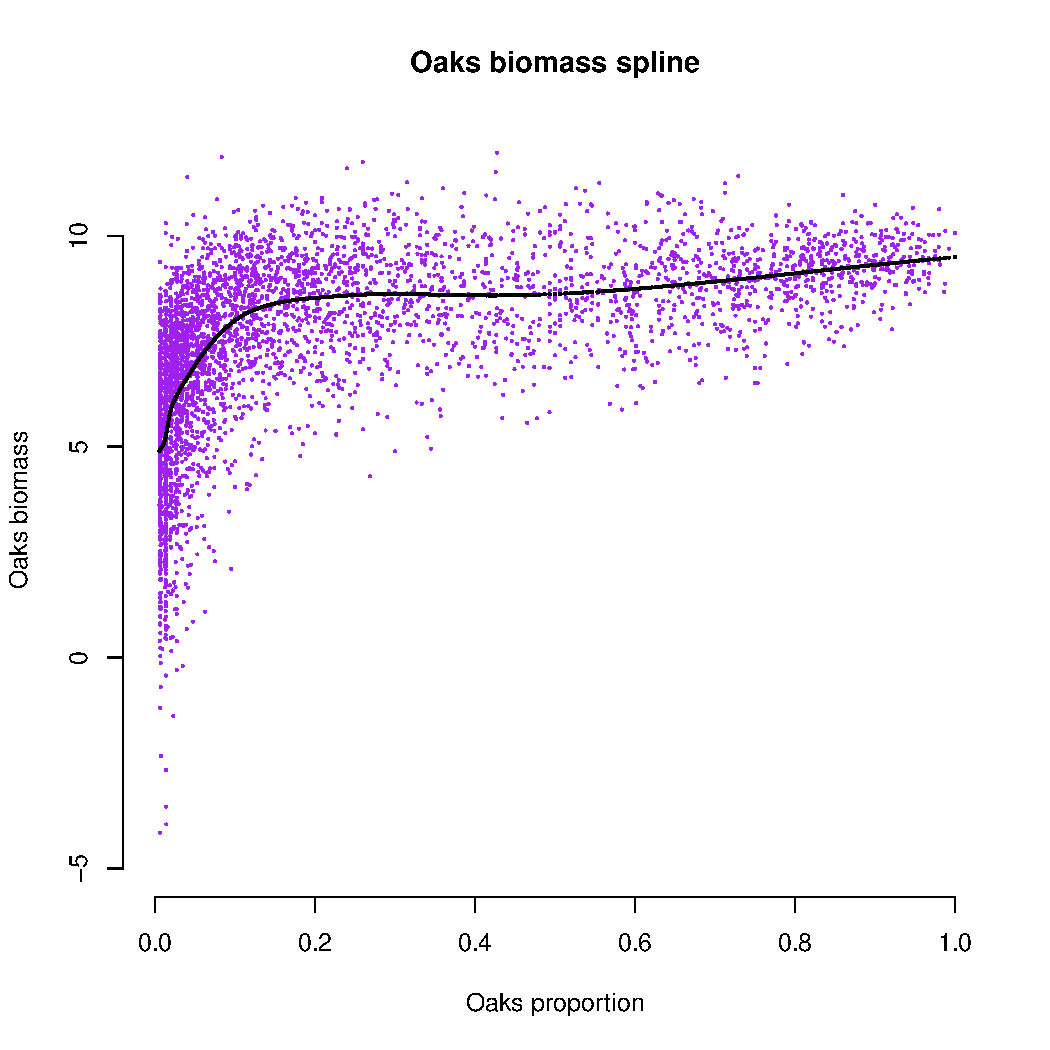
\includegraphics[width=5in]{../../figures/Oaks-biomass-spline.pdf}
	\end{center}
\end{figure}

\begin{figure}
	\begin{center}
	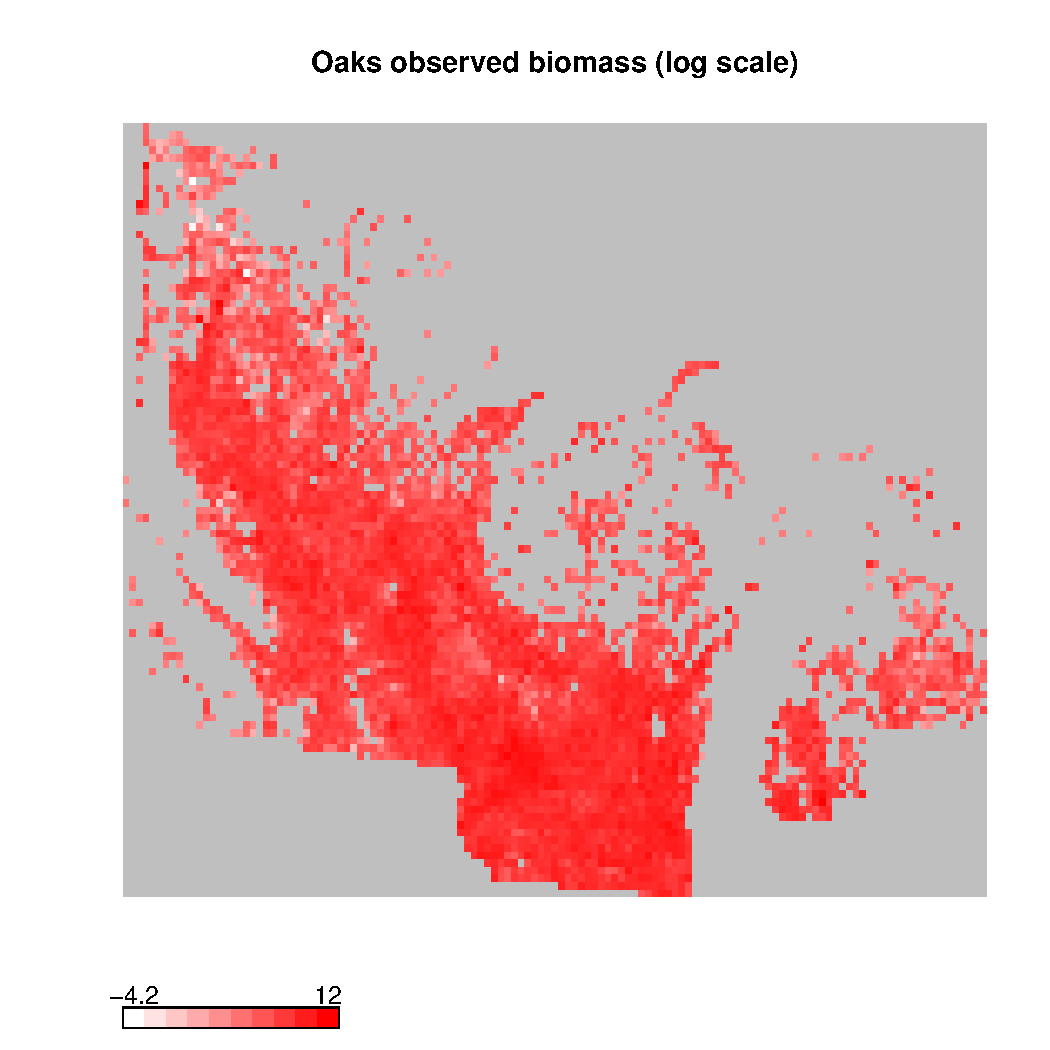
\includegraphics[width=5in]{../../figures/Oaks-biomass-observed.pdf}
	\end{center}
\end{figure}

\begin{figure}
	\begin{center}
	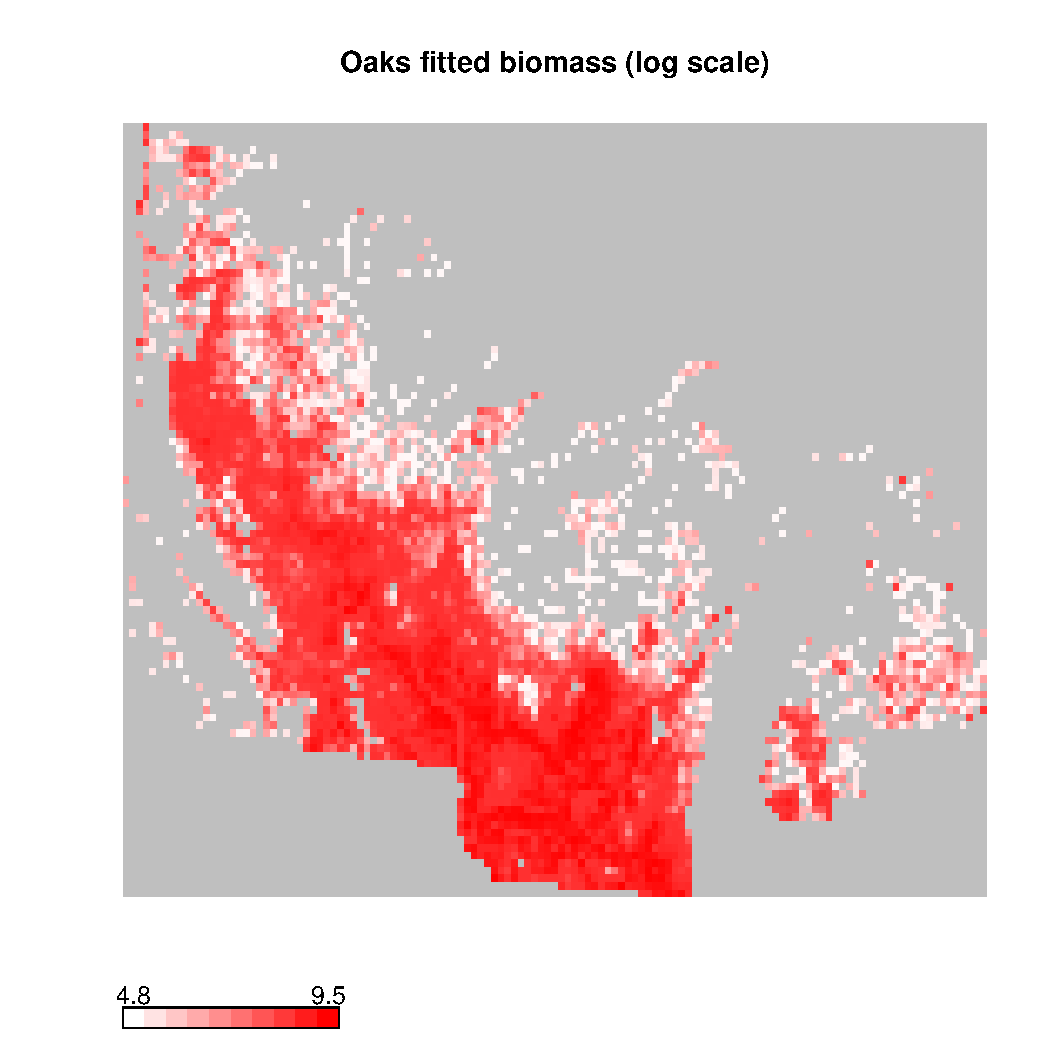
\includegraphics[width=5in]{../../figures/Oaks-biomass-fitted.pdf}
	\end{center}
\end{figure}

\begin{figure}
	\begin{center}
	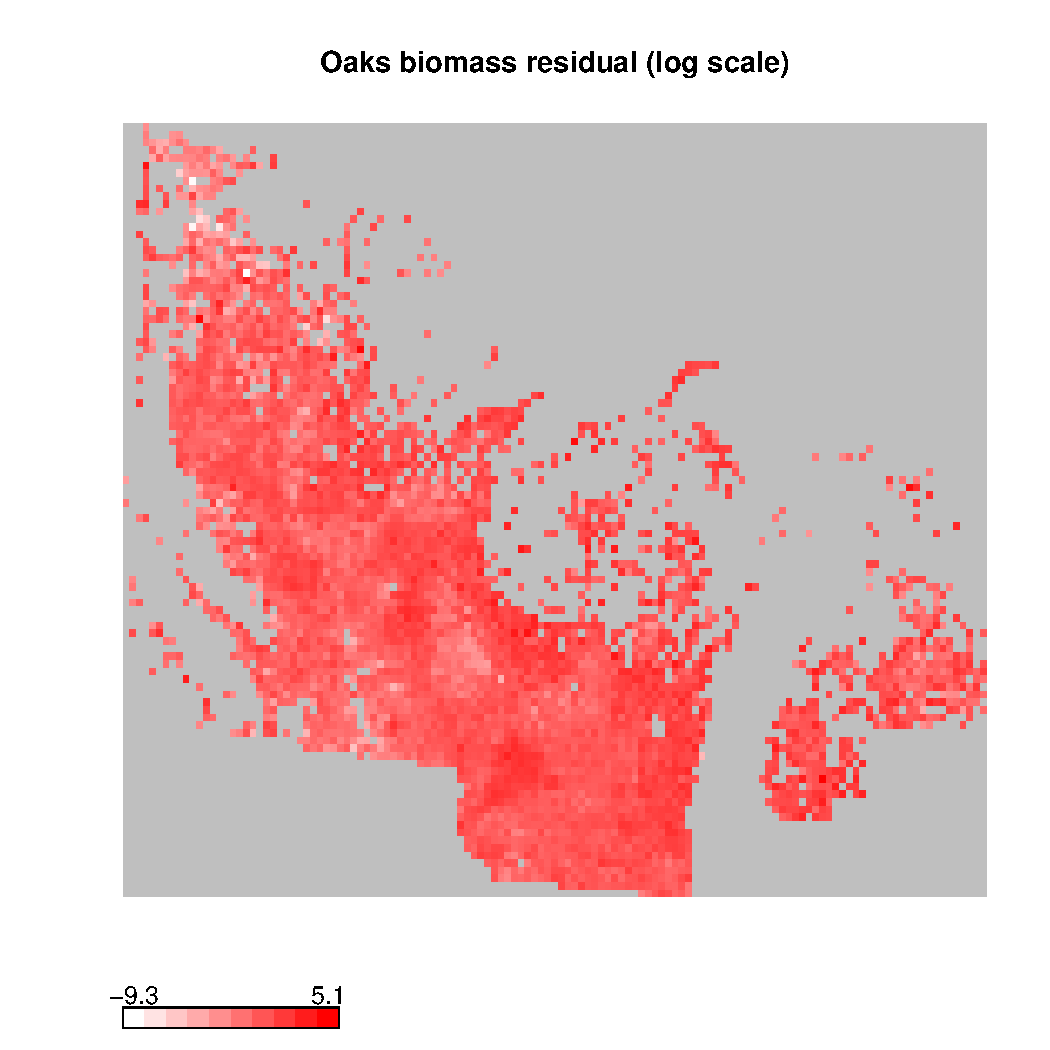
\includegraphics[width=5in]{../../figures/Oaks-biomass-residual.pdf}
	\end{center}
\end{figure}

\section{References}
%\bibliographystyle{chicago}
%\bibliography{../../references/biomass}

\end{document}  